\documentclass[12pt,twoside]{article}
\usepackage{../jmlda}
\usepackage{textcomp}

%\NOREVIEWERNOTES
\title
    [Локальные модели при декодировании сигналов головного мозга]
    {Исследование свойств локальных моделей при пространственном декодировании сигналов головного мозга.}
\author
    [Шиянов~В.\,А.]
    {Шиянов~В.\,А., Болоболова~Н.\,А., Самохина~А.\,М., Мокруполо~М.\,Н.}
\thanks
    {Работа выполнена при финансовой поддержке РФФИ, проект \No\,00-00-00000.
    Научный руководитель:  Стрижов~В.\,В.
    Задачу поставил: Стрижов~В.\,В.
    Консультант: Исаченко~Р.\,О.}
\email
    {vadimsh@phystech.edu}
%\organization
%    {$^1$Организация; $^2$Организация}
\abstract
    {Целью работы является восстановление связи между сигналами электрокортикограммы и пространственным движением конечностей тела.
    Особенностью является избыточность данных кортикограммы. Это позволяет снизить размерность задачи. В данном исследовании предлагается использовать пространственную информацию, то есть перемещение зон активности мозга. Для этого предлагается построить локальную модель описания сигнала и использовать ее параметры в качестве признакового описания.
    С помощью полученных признаков предлагается обучить алгоритм машинного обучения, который позволил бы предсказывать движения конечностей по сигналам головного мозга.
    В качестве данных предлагается использовать данные электрокортикограмм обезьян и движения их конечностей.

    \bigskip
    \textbf{Ключевые слова}: \emph{Brain-Computer Interface, feature engineering}.}
\begin{document}
\maketitle
\section{Введение}
Целью данной работы является построение модели, которая смогла бы связать сигналы мозга с движениями конечностей тела. Предлагается использовать пространственную составляющую сигнала, то есть перемещение зон активности головного мозга. Сложностью исследования является избыточное, высокоразмерное пространство сигналов, которое приводит к неустойчивой модели.\\
Для борьбы с высокой размерностью пространства признаков предлагается использовать ряд алгоритмов. В том числе PCA \cite{Jolliffe2011} для выделения наиболее важных признаков, то есть признаков, ответственных за наибольшую часть отклонения в выборке. Также предлагается использовать алгоритм PLS \cite{Haenlein2004} чтобы учесть латентную природу связей между сигналами головного мозга и движением тела. Также предлагается использовать алгоритм CCA \cite{thompson2005canonical} для выбора наиболее связанных из двух наборов переменных. Наиболее близкой к данной работе, является работа \cite{Motrenko_2018}. Эта работа также посвящена декодированию сигналов головного мозга и движения конечностей, однако, авторы ограничиваются частотными характеристиками сигналов.\\
Данное исследование предлагает использовать пространственную структуру сигнала. Для уменьшения размерности задачи предлагается построить локальную модель описания сигнала. Параметры этой модели предлагается использовать в качестве признакового описания сигнала. Такой подход позволяет заметно снизить размерность итоговых признаков, то есть позволяют построить более простую и устойчивую модель. Однако, результат построения локальной модели сильно зависит от изначального выбора признакового пространства, что влечет за собой ограничения на вид возмущения.\\
В работе предлагается использовать данные neurotycho (\url{http://neurotycho.org}), которые представляют из себя кортикограммы обезьян и движения их конечностей, записанные одновременно. С помощью этих данных предлагается обучить модель и проверить ее устойчивость и точность.

\section{Постановка задачи}
Данные электрокортикограммы содержат многомерные временные ряды $\mathbf{s}(t) \in \mathbb{R}^{N}$, представляющие измерения напряжения в каждом из $N$ каналов, а также временной ряд $\mathbf{y}(t) \in \mathbb{R}^3$, представляющий координаты конечности. Эти ряды можно представить в виде матриц $\mathbf{X} \in \mathbb{R}^{N \times T}$ и $\mathbf{Y} \in \mathbb{R}^{3 \times T}$ с элементами $x_{ij} = s_i(t_j)$ и $y_{ij} = y_i(t_j)$. Целью работы является создание модели
\[
    f: \mathbf{X} \to \mathbf{Y}.
\]
Так как $\mathbf{X}$ имеет большую размерность и содержит сильно зависимые данные, подобная модель может быть неустойчивой. Для решения этой проблемы предлагается признаковое описание сигнала в виде решения задачи линейной авторегрессии:
\[
    \left[\begin{array}{@{}c|ccc@{}}
        x_{i, t+1} & x_{i, t}   & \cdots & x_{i, t-n}   \\
        x_{i, t}   & x_{i, t-1} & \cdots & x_{i, t-n-1} \\
        \cdots     & \cdots     & \cdots & \cdots
    \end{array}\right]
    \begin{bmatrix}
        w_1 \\
        w_2 \\
        \cdots
    \end{bmatrix},
\]
где параметры $\mathbf{w}$ подбираются так, чтобы с помощью них можно было оптимально предсказывать первый зачения в первом столбце матрицы.\\
Таким образом модель $f$ разбивается на две: $g: \mathbf{X} \to \mathbf{w}$, которая ставит в соответствие сигналу его признаковое описание, и $h: \mathbf{w} \to \mathbf{Y}$, которая ставит в соответствие признакам движение конечности в пространстве. С помощью подобной декомпозиции задачи мы добиваемся сильного уменьшения размерности информации, что приводит к более устойчивым моделям $g$.\\
Формально постановку задачи можно записать следующим образом:
\[
    \mathbf{w}^* = \argmin_{\mathbf{w} \in \mathbb{R}^n} L(\mathbf{X}, \mathbf{Y}, \mathbf{w}, g, h)
\]
где $L$~--- некоторая функция потерь (например, cross-entropy или logloss).

\section{Базовый алгоритм}
Базовым алгоритмом в данной задаче является метод частичных наименьших квадратов (далее PLS).
Метод PLS относится к классу методов проекции на подпространства, которые предполагают поиск собственного базиса с последующим выбором в нем некоторого количества собственных векторов. Другие методы проекции на подпространства включают в себя метод главных компонент, линейный дискриминантный анализ и канонический корреляционный анализ. 

Метод PLS выгодно отличает то, что он позволяет одновременно выявлять скрытые связи между входными данными и аппроксимировать их. Более того, существуют реализации метода PLS, позволяющие построить регрессионную модель, описывающую зависимость между входными данными. 
Метод  PLS позволяет выделить из исходных данных компоненты, между которыми существует ковариационная связь. На основе этих компонент может быть построена модель регрессии. Такой подход позволяет не только существенно снизить вычислительные затраты, но и значительно улучшить точность модели по сравнению с линейной регрессией, построенной с помощью метода наименьших квадратов. 

\section{Метрики}
Для оценки качества предсказания использовались метрики mean squared error, mean absolute error и r2 score:
\[
  mse = \frac1n \sum_{i = 1}^n (y_i - \hat{y}_i)^2 \]\[
  mae = \frac1n \sum_{i = 1}^n |y_i - \hat{y}_i| \]\[
  r2 = 1 - \frac{\sum_{i = 1}^n (y_i - \hat{y}_i)^2}{\sum_{i = 1}^n (y_i - \overline{y})^2}
\]
Здесь $y_i$~--- предсказываемые данные, $\hat{y}_i$~--- предсказание модели, $\overline{y} = \frac1n \sum_{i = 1}^n y_i$~--- среднее $y_i$.

\section{Базовый эксперимент}
Для проведения эксперимента, из данных электрокортикограммы были выделены частоты сигналов. Выходные данные~--- трехмерные координаты движения руки обезьяны. Полученные данные были разделены на обучающую и контрульную выборки в отношении два к одному. На полученной выборке был обучен PLS с различным количеством компонент (от 2 до 100). Результаты эксперимента представлены на рис.~\ref{fig:baseAlgo}.
\begin{figure}
  \begin{center}
    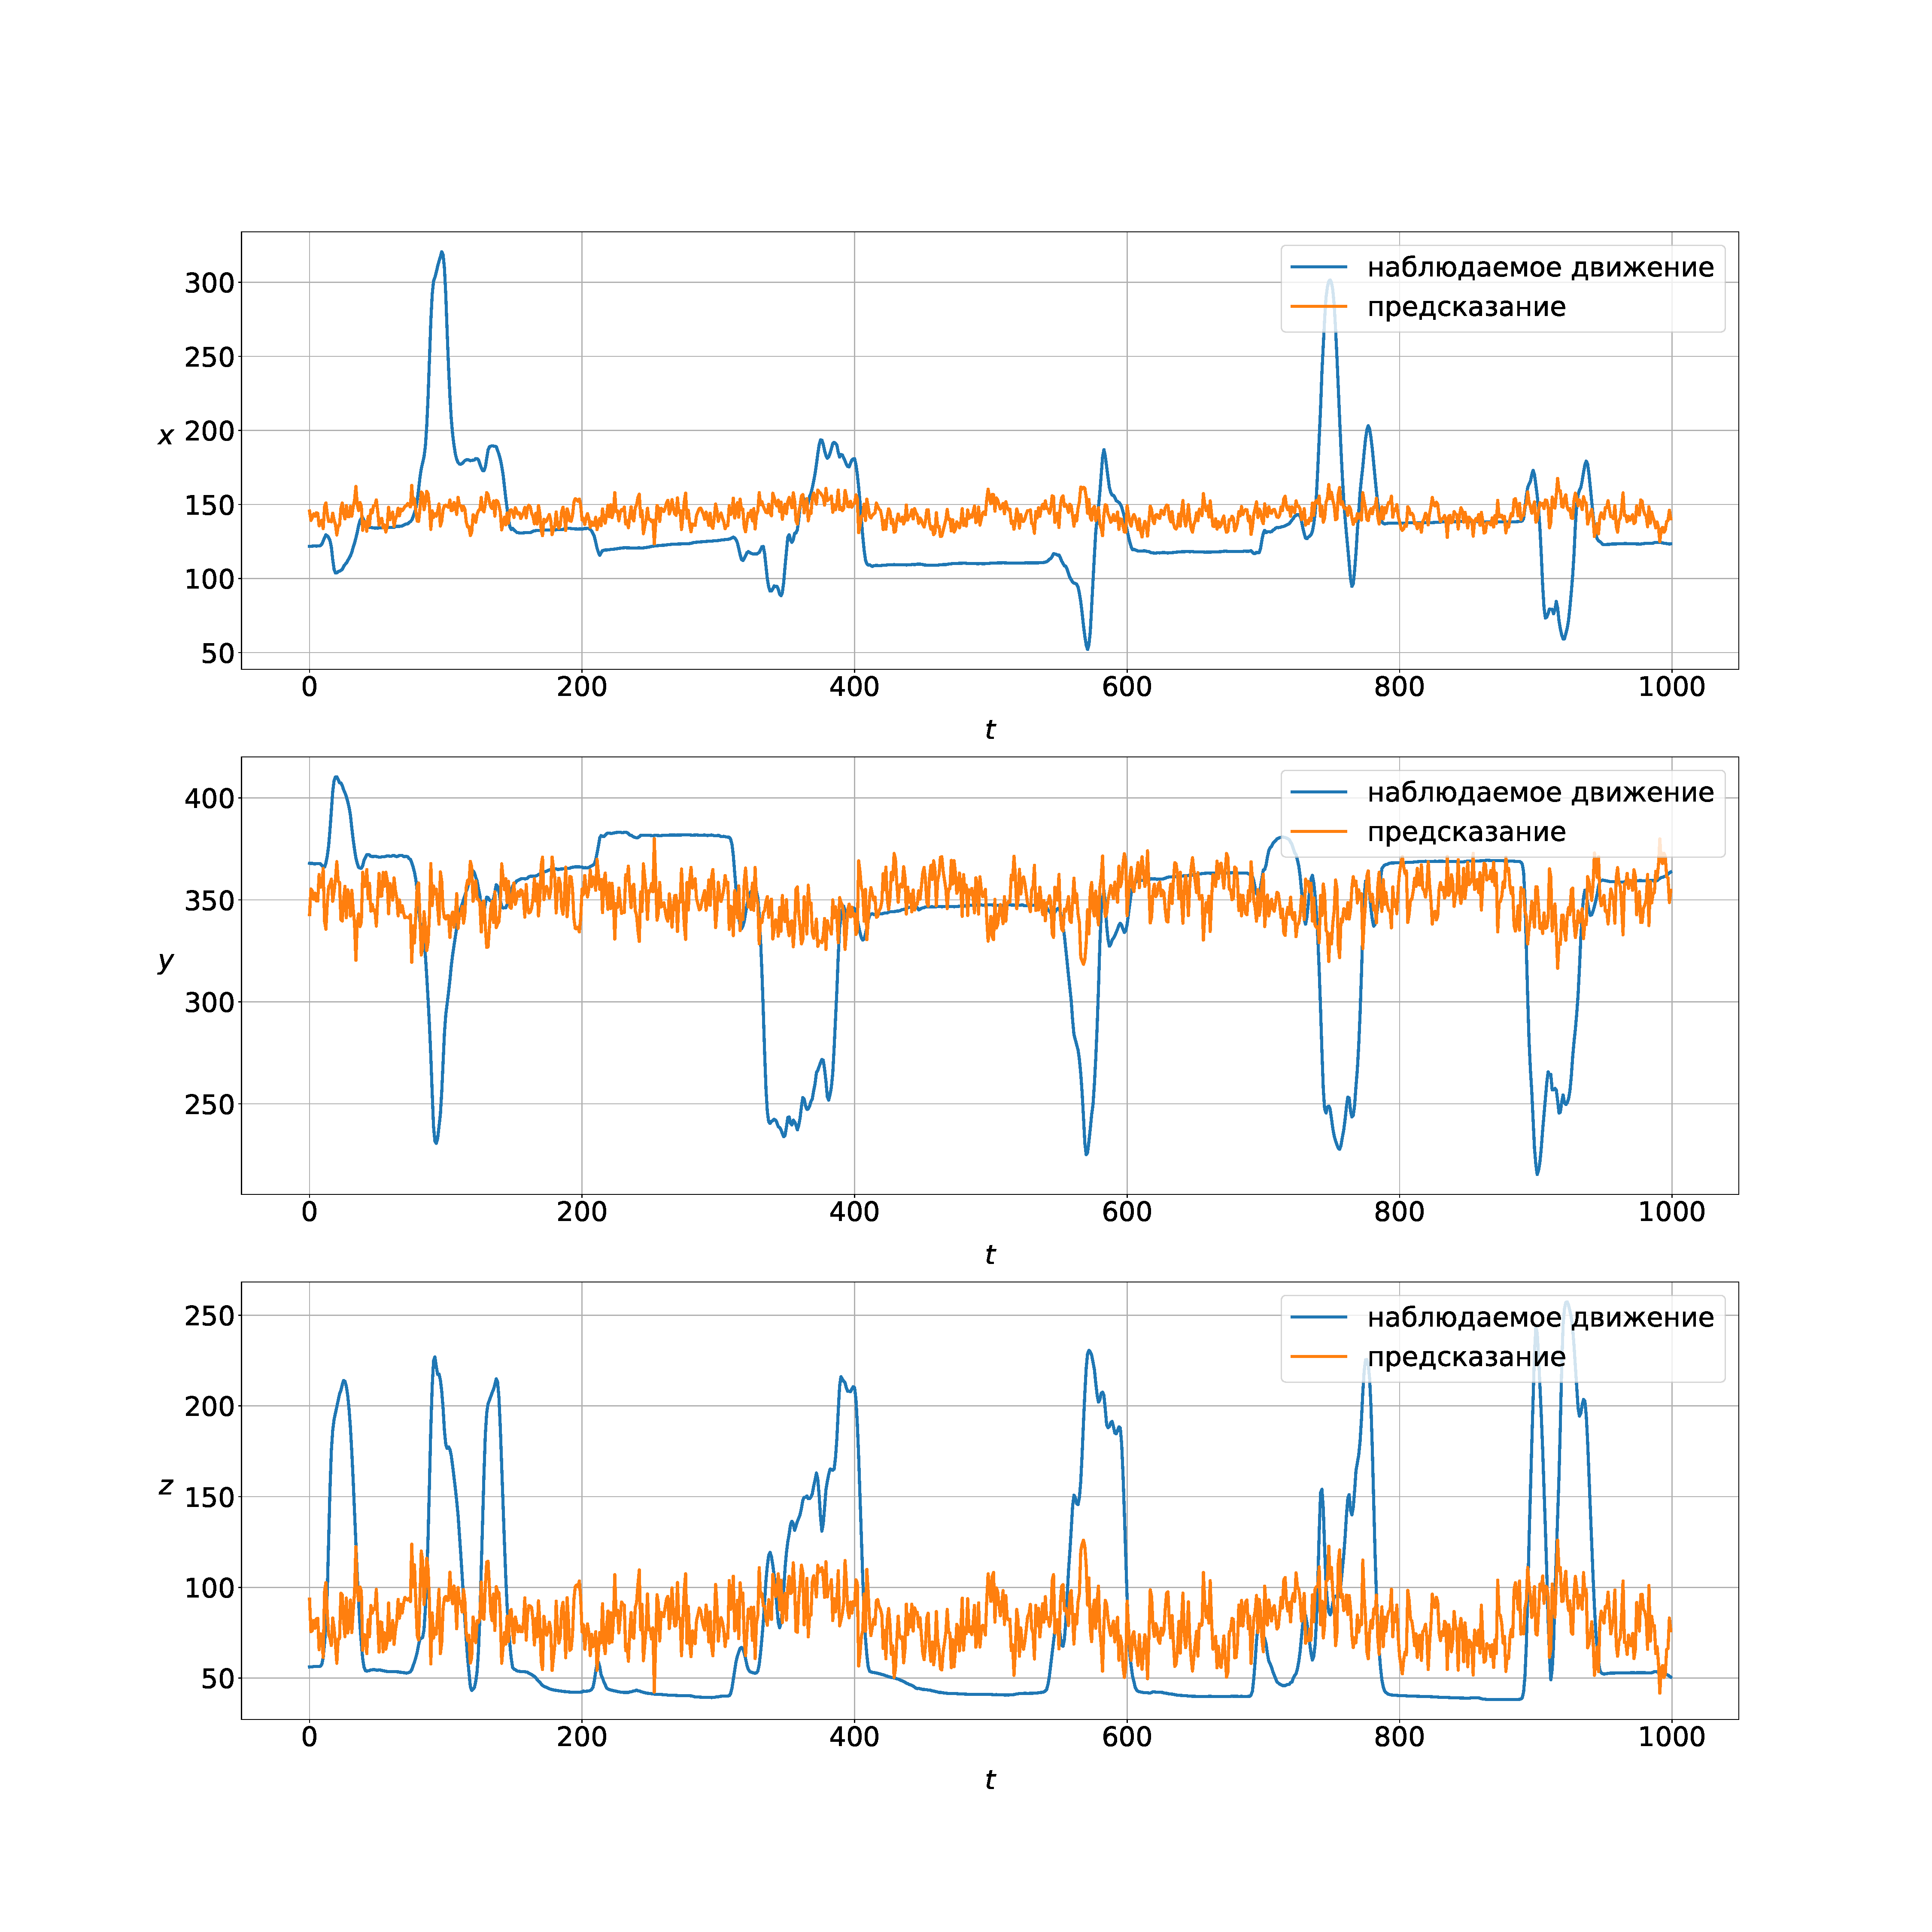
\includegraphics[width=\textwidth]{base_algo.pdf}
    \caption{Предсказания двухкомпонентного PLS, обученного на исходных данных}
    \label{fig:baseAlgo}
  \end{center}
\end{figure}
На графике представлена зависимость координаты конечности от времени. Как видно из рисунка, базовый алгоритм довольно плохо справляется с поставленной задачей. Общий профиль пиков соблюдается, однако PLS очень грубо оценивает острые пики. Также предсказание испытывает флуктуации, когда конечность почти не движется. В результате погрешность предсказания высока. Эксперимент показал значения метрик $mae = 30.17, mse = 1843.91, r2 = 0.01$. Для борьбы с погрешностями предлагается снизить размерность входного сигнала.


%\linenumbers
\bibliographystyle{plain}
\bibliography{../Project17}

\end{document}
